\documentclass{article}
\usepackage[utf8]{inputenc}
\usepackage[english]{babel}
\usepackage{graphicx}
\usepackage[a4paper, margin=1.2in]{geometry}
\usepackage[dvipsnames]{xcolor}
\usepackage{amsfonts}

\def\warning#1{\color{red} #1 \color{black}}
\def\note#1{\color{cyan} #1 \color{black}}
\def\acca#1{\color{OliveGreen} #1 \color{black}}
\def\accb#1{\color{Lavender} #1 \color{black}}
\def\accc#1{\color{Violet} #1 \color{black}}
\def\circled#1{\raisebox{.5pt}{\textcircled{\raisebox{-.9pt} {#1}}}}

\setlength{\parindent}{0mm}
\setlength{\parskip}{3mm}

\graphicspath{{./img/}}

\begin{document}

\title{Hoe los ik een examen Discrete Wiskunde op?}
\date{}
\author{Maestro Bert}
\maketitle

\tableofcontents


Het examen Discrete Wiskunde verandert weinig en bestaat altijd uit zeven vragen. Zes van deze vragen zijn analoog met elke examenperiode en één vraag is willekeurig vanuit heel de cursus. In dit document wil ik technieken toelichten om het examen op een goede manier op te lossen. Dit gaat vooral over trukjes in Excel en de Antiview die je kan gebruiken in plaats van alles manueel te doen. 

De voorbeelden zijn beschikbaar in het mapje \textit{excel}. In de tekst zal naar deze bestanden gerefereerd worden. Verder wordt ook nog het examen van januari 2018 opgelost in dit document.
 
\section{Velden}
\subsection{Het algoritme van Euclides}
Het algoritme van Euclides komt bij vele onderwerpen terug en moet goed gekend zijn. Het is handig om Excel het meeste werk te laten doen. Het bestand \texttt{algo\_euclides.xlsx} bevat 2 voorbeelden van dit algoritme. De betekenis van hun resultaat wordt later toegelicht. 

Het algoritme van Euclides bepaalt de grootst gemene deler van 2 gehele getallen. Deze bewerking wordt afgekort tot $ggd(A,B)$. Het eerste voorbeeld stelt $ggd(53, 97)$ voor en het tweede voorbeeld stelt $ggd(6, 18)$ voor. Voorbeeld 1 wordt volledig toegelicht.

De waarde 53 komt in de cel $A3$ te staan terwijl de waarde 97 in de cel $C4$ komt. Daarna typ je in de cel $B4$ het volgende: \texttt{=FLOOR.MATH(A3/C4)}. We gebruiken de floor-functie omdat we geïnteresseerd zijn hoeveel keer 97 in 53 past. In cel $A4$ doe je nu de vermenigvuldiging met de waarde 97 en het aantal keer dat deze in 53 past: \texttt{=C4*(-B4)}. We gebruik het minteken bij B4 zodat we een negatief getal krijgen in $A4$ (nu niet want het is 0). Op die manier is het eenvoudiger te zien dat we later cijfers aftrekken. In cel $A5$ tel je nu de twee bovenste cellen op: \texttt{=A3 + A4}. 

Nu wordt er in omgekeerde volgorde gewerkt. In cel $B5$ zetten we de formule \texttt{=FLOOR.MATH(C4/A5)} en in cel $C5$ zetten we \texttt{=A5*(-B5)}. In cel $C6$ steken we nu de som van de twee bovenste cellen: \texttt{=C4 + C5}.

Op dit moment is de basisopstelling klaar. Indien je nog geen 0 uitgekomen bent kan je nu doorslepen. Selecteer de range $[A4:B5]$ en sleep een aantal cellen door. Doe dit hetzelfde met de range $[C5:C6]$. Merk op dat de tweede range een cel lager begint en je beide ranges dus niet kunt combineren. Blijf dit doen totdat je een 0 uitkomt in ofwel de linkerkolom of in de rechterkolom.

Op het moment dat je een 0 tegenkomt mag je stoppen. Het vorige element (het groen gekleurde) is gelijk aan $ggd(53, 97)$. Merk op dat de inkleuring niet gebeurd en je dus zelf moet doen. Het klopt dat $ggd(53, 97) = 1$ want zowel 53 als 97 zijn priemgetallen. Bij het tweede voorbeeld krijgen we $ggd(6, 18) = 6$, wat zondermeer duidelijk is.
\subsubsection{Veralgemeende algoritme van Euclides}
Het veralgemeende algoritme van Euclides is een uitbreiding op het normaal algoritme van Euclides. Het heeft 2 zaken van praktisch nut:

\begin{itemize}
 \item Het controleert of het normale algoritme van Euclides correct uitgevoerd is
 \item De multiplicatieve inverse kan bepaald worden met het veralgemeende algoritme van Euclides
\end{itemize}


\subsection{Berekenen van een primitieve wortel}
Een primitieve wortel is het kleinste getal dat niet deelbaar is door een bepaald getal voor een bepaald veld. Het berekenen van een primitieve is heel eenvoudig. 
Er is slechts één gegeven nodig en dat is het veld. We nemen het volgende voorbeeld: Bereken de primitieve wortel over $\mathbb{Z}_{271}.$

\begin{enumerate}
 \item Trek 1 af van het veldgetal en ontbindt dit in factoren. Gebruik het programma {\it factor} dat ook beschikbaar is op het examen. (Ingeven: {\sl factor 270}) 
  $$271- 1 = 270 = 2 * 3^3 * 5$$
  Het getal 270 wijst simpelweg op het aantal elementen in dit veld.
 \item We hebben het getal 270 ontbonden in factoren. De bedoeling is om een excel-bestand op te maken zodat de primitieve wortel redelijk eenvoudig kan berekend worden. Dit kan teruggevonden worden in \texttt{primitieve\_wortel.xlsx}

 In vak \texttt{B2} bevindt zich het veldgetal. Stel het drie-dimensionaal rooster op (aangezien 270 ontbonden wordt in 3 priemfactoren). Begin altijd met $x$. Voeg daarna zoveel rijen toe als de macht die bij de kleinste priemfactor staat. In dit geval is het $2^1$, dus voeg één rij toe. Dit is rij \texttt{6} in het excelbestand. Voeg nu in rij 5 zoveel kolommen toe als de macht die bij de tweede kleinste priemfactor staat. Dit is $3^3$, dus 3 extra kolommen. Voeg aan alle andere rijen ook deze kolommen toe. Nu hebben we een 2-dimensionaal rooster met 2 rijen en 4 kolommen. Om daarna nog de derde dimensie toe te voegen kopieër je gewoon het origineel rooster, en je voegt daar de hoogste priemfactor aan toe. 
 
 Wanneer het rooster klaar is begin je met x=2 (je moet wel nog eens apart in excel zelf de formules doen), en blijf je x incrementeren met 1 totdat enkel de hoogste macht (in dit geval $x^{2*27*5}$) het getal 1 bevat. De $x$ waarvoor dit geldt is de kleinste primitieve wortel. In dit voorbeeld is $x = 6$ de primitieve wortel.
 \end{enumerate}

 
 \subsection{De baby-step, giant-step techniek}
 De baby-step, giant-step techniek wordt gebruikt om een index van een getal ten opzichte van een primitieve wortel in een bepaald veld te berekenen. Hier moet de Euclidische deling ook uitgevoerd worden dus zorg dat je dit al goed kunt. Bij dit soort vraagstukken zijn er 3 gegevens.
 \begin{itemize}
  \item {Het veld $\mathbb{Z}$.} 
  \item {Een getal in dit veld waarvan de index moet berekend worden.}
  \item {De primitieve wortel $w$.}
 \end{itemize}
 Op het examen zal er staan hoe groot één giant-step moet zijn. In dit voorbeeld nemen we giant-steps die 10 baby-steps groot zijn. We beschouwen het veld $\mathbb{Z}_{71}$ en de primitieve wortel $w = 7$. We willen de index van 5 berekenen. Begin met de eerste 10 baby-steps te genereren. Je begint met de primitieve wortel, en daarna gebruik je Formule 1. De letter b stelt de n-de baby-step voor. Bekijk ook Figuur \ref{fig:babystep_giantstep_1} waarop dit gevisualiseerd staat(p. \pageref{fig:babystep_giantstep_1}).
 $$b_n = b_{n-1} * w\; \% \;71 \eqno(1)$$
 
\begin{figure}
  \begin{center}
  \caption{Voorstelling van Formule 1 voor de berekening van de baby-steps}
  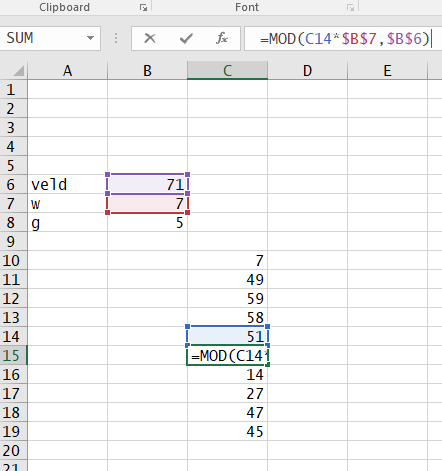
\includegraphics[width=\textwidth]{babystep_giantstep_1}
  \label{fig:babystep_giantstep_1}
  \end{center}
  
\end{figure}
  
 
Nadat de eerste 10 baby-steps genereerd zijn moet je het inverse element, ten opzichte van 71, van de laatste baby-step bepalen. Dit doe je door het algoritme van Euclides toe te passen(Figuur \ref{fig:babystep_giantstep_2}).

\begin{figure}
  \begin{center}
  \caption{Algoritme van Euclides bij de baby-step, giant-step techniek}
  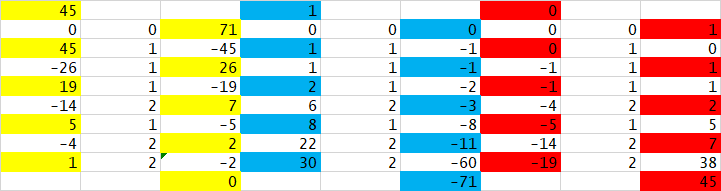
\includegraphics[width=\textwidth]{babystep_giantstep_2}
  \label{fig:babystep_giantstep_2}
  \end{center}
\end{figure}
Het inverse element is hier dus 30. Nu moeten de giant-steps gegenereerd worden. Je vertrekt vanaf het getal waarvan we de index zoeken. Daarna gebruik je Formule 1 maar vervang je de baby-step door de giant-step. Dit wordt voorgesteld in Figuur \ref{fig:babystep_giantstep_3}.


\begin{figure}
  \begin{center}
  \caption{Voorstelling van Formule 1 voor de berekening van de giant-steps}
  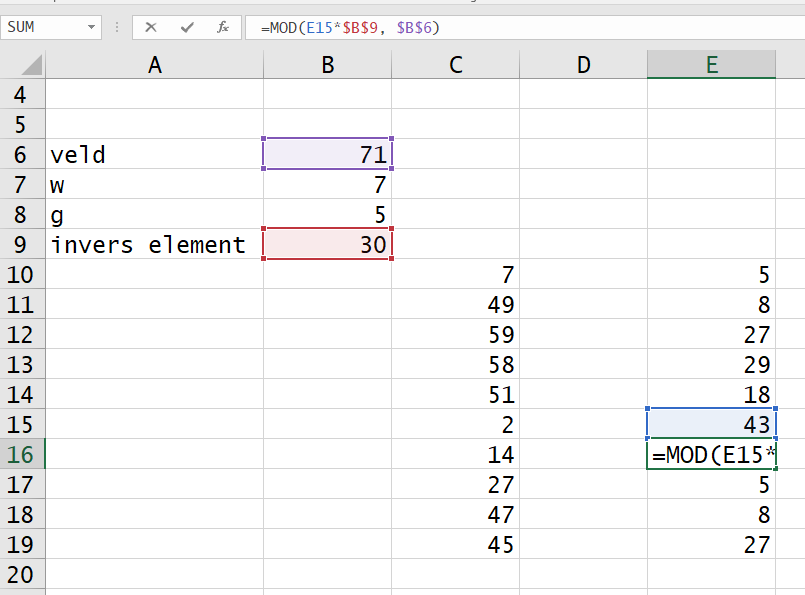
\includegraphics[width=\textwidth]{babystep_giantstep_3}
  \label{fig:babystep_giantstep_3}
  \end{center}
\end{figure}
  
Merk op dat het getal 27 zowel bij de baby-steps als bij de giant-steps voorkomt. Dit stelt de index voor die we zoeken. Het getal 27 is het achtste getal in de baby-step verzameling. Bij de giant-step verzameling is dit het derde getal. Aangezien elke giant-step een grootte heeft van tien babysteps, wordt dit nog eens vermenigvuldigd met tien. De index wordt $$8 + (3 * 10) = 8 + 30 = 38$$
De oplossing is formeel: De index van 5 over het veld $\mathbb{Z}_{71}$ met primitieve wortel $w = 7$ is 38. Er zijn 3 giant-steps en 8 baby-steps nodig.

\subsection{Irreducibele veeltermen}
Een irreducibele veelterm is een veelterm dat niet meer deelbaar is over een bepaald veld. Op het examen wordt een priemveld gegeven en een bepaalde veelterm. Om te bepalen hoeveel veeltermen hiervan irreducibel zijn kan volgende formule gebruikt worden: 

$$\frac{1}{n} \sum_{d|n} \mu(d) \cdot p^{n/d}$$ 

met $\mu(d)$ de Mobius $\mu$ (Zie slide 3 van \texttt{1b.pptx})


Voor $F_{32}$ ( p = 2, n = 5 ) komen we uit:

$$\frac{1}{5} \bigg( \mu(1) \cdot p^{5/1} + \mu(5) \cdot p^{5/5} \bigg) = \frac{1}{5} ( p^5 - p ) = 6$$

BOm nu na te gaan of een bepaalde veelterm irreducibel is moet een test uitgevoerd worden met elke veelterm $x^{\acca{p}^{\accb{i}}} - x$ met $\accb{i} \leq \frac{\accc{n}}{2}$. Het komt erop neer dat je $n$ deelt door 2 en dit getal afrond naar beneden. Dus $floor(\frac{\accc{5}}{2}) = 2$. 

De test moet dus uitgevoerd worden met $\accb{i = 1}$ en $\accb{i = 2}$. We moeten de veelterm  dus delen door $x^{\acca{2}^{\accb{1}}} - x$ en $x^{\acca{2}^{\accb{2}}} - x$. Indien geen gemeenschappelijke deler werd gevonden dan is de veelterm irreducibel. Je kan eenvoudig de euclidische deling uitvoeren. Je moet enkel elke graad als een 'getal' zien. Zo is $4x^3 + x + 7$ gelijk aan $4017$. We gaan na of de veelterm $x^4 + x + 1$ irreducibel is in $F_{32}$. De uitwerking is terug te vinden in \texttt{irreducibele\_veelterm.xlsx}.

Je moet bij de euclidische deling nu werken met graden in plaats van gewoon getallen. In vak \texttt{C5} vermenigvuldigen we met \'100'. Eigenlijk is dit gelijk aan $x^2$. Dus $x^2 + x$ vermenigvuldigen met $x^2$ geeft $x^5 + x^4$ wat overeenkomt met 11000. Als voor alle delingen een 1 als resultaat opleveren, dan is de opgegeven veelterm irreducibel.


\subsection{Elliptische krommen}
Bij een vraag over een elliptische kromme krijg je zeker drie gegevens:
\begin{enumerate}
 \item Het veld en de vergelijking van de elliptische kromme
 \item De irreducibele veelterm
 \item De primitieve wortel
 \item Een groepstabel
\end{enumerate}

Op het examen worden er slides gegeven (meer specifiek, slide 6 en 10 van het bestand 1d.pptx). Dit zijn de slides waarop de berekening voor het verdubbelen van de punten opstaan, dus deze moet je niet  vanbuiten kennen. Je moet wel weten welke slide je nodig hebt, maar dit is gewoon naar de vergelijking kijken en zien welke er overeenkomt met die op de slide. Voor de verdere uitwerking van dit onderdeel worden de gegevens van het examen gebruikt.



\subsubsection{Berekening van de punten}
De eerste stap is altijd het berekenen van alle punten op deze elliptische kromme. 

\subsubsection{Verdubbeling van de punten}

\subsubsection{Soort bepalen}

\section{Grafen}


\warning{pr\"ufercode}

\warning{boogkleuring}

\warning{hongaarse methode}

\warning{algoritme x}

\section{Groepen}
\subsection{Partitionering van de groepselementen in conjugatieklassen}
\subsection{Cykelindex bepalen}
Op het examen wordt er gevraagd om de cykelindex van een willekeurige drie dimensionele veelhoek te bepalen. Daarna wordt er gevraagd om het aantal configuraties te bepalen waarbij een X aantal kleuren Y maal gebruikt worden.

Op deze vraag moet de AntiView gebruikt worden die standaard al open staat op het examen met de figuur. Dit programma toont default de symmetrie en rotatie-assen niet. Zonder dit hulpmiddel is deze vraag haast onmogelijk. Je kan de assen tonen door op de knop 'Y' te drukken op het toetsenbord. In de voorbeelden gebruiken we een kubus. Je kan deze figuur ook bekomen door het programma AntiView via de commandolijn op te starten met als argument \texttt{cube}.

\begin{center}
 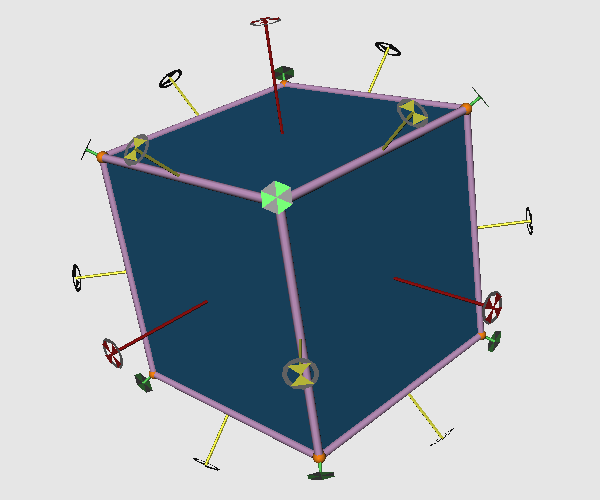
\includegraphics[width=\linewidth]{antiview_cube_1}
\end{center}

Normaal zie je 3 soorten assen verschijnen: rode, gele en groene. Elke kleur heeft zijn eigen betekenis.
\begin{itemize}
 \item \textbf{Rood}:
 \item \textbf{Geel}:
 \item \textbf{Groen}:
\end{itemize}



\section{Voorbeeldexamen}





\end{document}
